\chapter{Multimodal Enriched Audio Generation}

\begin{tcolorbox}[colback=DarkSkyBlue!5!white,colframe=DarkSkyBlue!75!black,title=Chapter Summary]
This chapter presents a mathematical framework for multimodal audio generation within the Elder Heliosystem, describing approaches for integrating diverse input modalities to synthesize contextually appropriate audio outputs. We examine mathematical models for the integration of audio, visual, and semantic features through orbital dynamics, analyze representations of cross-modal information flow coherence during generation, where information flow coherence refers to the synchronized propagation of semantic content across multiple modalities while maintaining phase relationships and causal dependencies, and discuss theoretical aspects of generation quality in relation to multimodal input characteristics. The chapter explores tensor-based formulations for audio generation from multimodal conditioning signals, examines properties of cross-modal resonance related to audio-visual synchronization, and compares this approach with other generation methods. Through mathematical analysis, we examine how multimodal generation within the Elder Heliosystem relates to its architectural principles: hierarchical decomposition corresponding to different levels of audio structure from timbral details to high-level form, phase relationships relating to temporal consistency, orbital dynamics addressing conditional generation based on multimodal inputs, and resonance phenomena affecting cross-modal synchronization. This theoretical framework contributes to understanding multimodal audio generation within the Elder paradigm, examining approaches for creating audio with internal coherence and appropriate relationships to conditioning information from other modalities.
\end{tcolorbox}

\section{Elder Heliosystem Configuration for Enriched Audio Generation}

High-fidelity audio generation from multimodal features requires a specialized Elder Heliosystem configuration that efficiently processes and integrates diverse input modalities. This chapter details the precise architectural design for processing enriched audio data with accompanying video-extracted features and semantic content descriptors.

\subsection{System Architecture Overview}

The Elder Heliosystem for multimodal audio generation uses a hierarchical orbital configuration with domain-specialized Mentors and feature-specialized Erudites:

\begin{table}[h]
\centering
\begin{tabular}{|l|c|l|}
\hline
\textbf{Component} & \textbf{Quantity} & \textbf{Role Description} \\
\hline
Elder & 1 & Maintains global coherence across all modalities \\
\hline
Mentors & 32 & Domain specialists (audio, visual, semantic, temporal, spatial, etc.) \\
\hline
Erudites & 4,096 & Feature-specific processing units \\
\hline
\end{tabular}
\caption{Elder Heliosystem Component Configuration}
\end{table}

\subsection{Orbital Configuration for Multimodal Processing}

The orbital arrangement of this specialized Elder Heliosystem follows a multimodal integration pattern:

\begin{figure}[h]
\centering
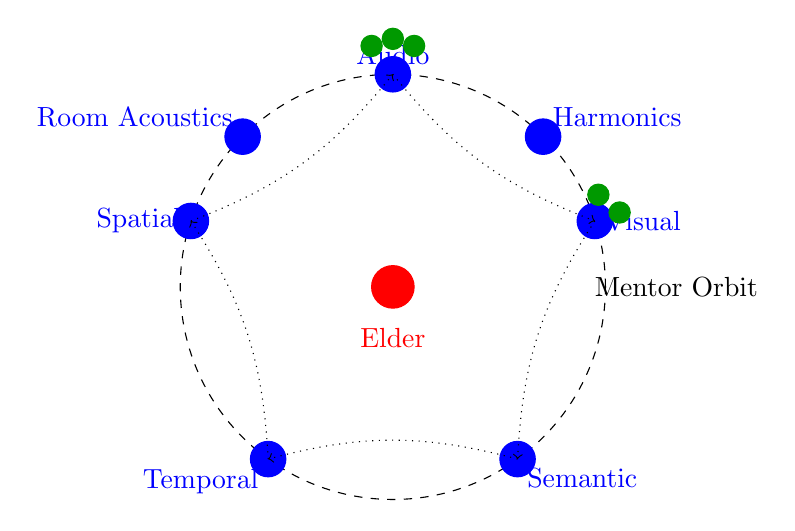
\begin{tikzpicture}[scale=0.9]
% Elder at center
\filldraw[red] (0,0) circle (0.3) node[below=0.4cm] {Elder};

% Mentor orbits
\draw[dashed] (0,0) circle (3);

% Core domain Mentors (on main orbit)
\filldraw[blue] (0,3) circle (0.25) node[above] {Audio};
\filldraw[blue] (2.85,0.93) circle (0.25) node[right] {Visual};
\filldraw[blue] (1.76,-2.43) circle (0.25) node[below right] {Semantic};
\filldraw[blue] (-1.76,-2.43) circle (0.25) node[below left] {Temporal};
\filldraw[blue] (-2.85,0.93) circle (0.25) node[left] {Spatial};

% Other specialized Mentors
\filldraw[blue] (2.12,2.12) circle (0.25) node[above right] {Harmonics};
\filldraw[blue] (-2.12,2.12) circle (0.25) node[above left] {Room Acoustics};

% Erudites (selected)
\filldraw[green!60!black] (0,3.5) circle (0.15);
\filldraw[green!60!black] (0.3,3.4) circle (0.15);
\filldraw[green!60!black] (-0.3,3.4) circle (0.15);
\filldraw[green!60!black] (3.2,1.05) circle (0.15);
\filldraw[green!60!black] (2.9,1.3) circle (0.15);

% Labeled orbit
\node at (4,0) {Mentor Orbit};

% Cross-modal connections
\draw[dotted, ->] (0,3) to[bend right=15] (2.85,0.93);
\draw[dotted, ->] (2.85,0.93) to[bend right=15] (1.76,-2.43);
\draw[dotted, ->] (1.76,-2.43) to[bend right=15] (-1.76,-2.43);
\draw[dotted, ->] (-1.76,-2.43) to[bend right=15] (-2.85,0.93);
\draw[dotted, ->] (-2.85,0.93) to[bend right=15] (0,3);

\end{tikzpicture}
\caption{Elder Heliosystem Orbital Configuration for Multimodal Audio Generation}
\end{figure}

\subsection{Multimodal Feature Integration}

The system processes enriched feature sets across multiple domains:

\begin{table}[h]
\centering
\small
\begin{tabular}{|l|p{5.5cm}|l|l|}
\hline
\textbf{Domain} & \textbf{Features} & \textbf{Resolution} & \textbf{Mentor Phase} \\
\hline
Audio & Spectral centroid, MFCC, chroma, onset strength, pitch contours & 44.1/96kHz, 10-40ms frames & $\phi_A = 0.0$ \\
\hline
Visual & Object positions, motion vectors, scene composition, lighting, depth maps & 256×256 to 1024×1024, 30-60fps & $\phi_V = 1.257$ \\
\hline
Semantic & Object labels, action descriptions, emotional content, narrative context & Variable length embeddings & $\phi_S = 2.513$ \\
\hline
Temporal & Event boundaries, rhythmic patterns, scene transitions, causal relationships & Multiple timescales (ms-min) & $\phi_T = 3.770$ \\
\hline
Spatial & Room dimensions, acoustic properties, object positions, spatial audio cues & 3D coordinates, reverb params & $\phi_{Sp} = 5.027$ \\
\hline
\end{tabular}
\caption{Multimodal Feature Set with Phase Assignments}
\end{table}

\subsection{Phase Relationships for Cross-Modal Integration}

Cross-modal integration is facilitated by precise phase relationships between the Elder and domain-specific Mentors:

\begin{equation}
\phi_{E \to M_i} = \phi_E + \frac{2\pi \cdot i}{N_M} \quad \text{for } i \in \{0,1,\ldots,N_M-1\}
\end{equation}

where $N_M = 32$ is the total number of Mentors, with core modality Mentors at specific phase positions. The Elder phase $\phi_E$ evolves according to:

\begin{equation}
\frac{d\phi_E}{dt} = \omega_E + \sum_{i=0}^{N_M-1} \alpha_i \cdot \mathcal{F}_i(t) \cdot \sin(\phi_{M_i} - \phi_E)
\end{equation}

where $\mathcal{F}_i(t)$ represents the feature salience for Mentor $i$ at time $t$, and $\alpha_i$ is the coupling strength for that Mentor's domain.

\subsection{Entity State Configuration for Enriched Audio}

The optimized entity state configuration for multimodal audio generation includes:

\begin{figure}[h]
\begin{center}
\begin{minipage}{0.95\textwidth}
\begin{verbatim}
// MultimodalEntityState extends the optimized entity state
// for cross-modal feature processing
type MultimodalEntityState struct {
    // Base optimized entity state
    OptimizedEntityState
    
    // Domain specialization
    DomainID        uint8      // Domain identifier
    FeatureType     uint16     // Specific feature type within domain
    
    // Feature integration parameters
    CrossModalGain  [5]uint8   // Per-domain integration weights
    TemporalContext uint16     // Temporal context window size
    
    // Activation thresholds for different feature types
    FeatureThreshold [8]uint8  // Activation thresholds per feature type
    
    // Coupling coefficients
    PhaseCouplingSelf float16   // Self-coupling coefficient
    PhaseCouplingElder float16  // Elder coupling coefficient
    PhaseCouplingCross float16  // Cross-modal coupling coefficient
    
    // Total: 29B (base) + 24B (multimodal) = 53B per entity
}
\end{verbatim}
\end{minipage}
\caption{Extended Entity State for Multimodal Processing}
\end{center}
\end{figure}

\subsection{Modal Coupling Tensors}

The system uses specialized coupling tensors to model interactions between different modalities:

\begin{equation}
\mathcal{T}_{ijk} \in \mathbb{C}^{N_A \times N_V \times N_S}
\end{equation}

where $N_A$, $N_V$, and $N_S$ are the dimensions of the audio, visual, and semantic feature spaces, respectively. The coupling tensor $\mathcal{T}$ is highly sparse with a sparsity factor of $s = 10^{-5}$, and elements are stored in polar form:

\begin{equation}
\mathcal{T}_{ijk} = \rho_{ijk}e^{i\phi_{ijk}}
\end{equation}

This representation enables efficient storage and computation, as only non-zero elements are stored, with their phases indexed for rapid retrieval based on the Elder phase.

\subsection{Phase-Based Feature Selection}

For high-fidelity audio generation, the system performs phase-based feature selection to determine which multimodal features influence the current audio frame:

\begin{figure}[h]
\begin{center}
\begin{minipage}{0.95\textwidth}
\begin{verbatim}
// SelectActiveFeatures determines which multimodal features are active
// based on the current Elder phase
func SelectActiveFeatures(elderPhase float32, features []FeatureVector) []bool {
    activeFeatures := make([]bool, len(features))
    activeCount := 0
    
    for i, feature := range features {
        // Calculate phase distance (accounting for circular phase)
        phaseDist := MinCircularDistance(feature.Phase, elderPhase)
        
        // Feature-type specific thresholds
        threshold := GetThresholdForType(feature.Type)
        
        // Apply salience-based modulation to threshold
        modThreshold := threshold * (0.5 + 0.5*feature.Salience)
        
        // Feature is active if within phase threshold
        activeFeatures[i] = phaseDist < modThreshold
        
        if activeFeatures[i] {
            activeCount++
        }
    }
    
    // Dynamic threshold adjustment based on context
    if activeCount < MinRequiredFeatures || activeCount > MaxAllowedFeatures {
        AdjustThresholds(activeCount)
        return SelectActiveFeatures(elderPhase, features)
    }
\end{verbatim}
\end{minipage}
\caption{Multimodal Feature Selection Algorithm}
\end{center}
\end{figure}
    


\subsection{Cross-Modal Audio Generation Flow}

The process flow for generating high-fidelity audio from enriched multimodal features follows these steps:

\begin{algorithm}
\caption{Elder Heliosystem Multimodal Audio Generation}
\begin{algorithmic}[1]
\State \textbf{Input:} Enriched feature set $\mathcal{F}$ containing audio, visual, semantic, temporal, and spatial features
\State \textbf{Output:} High-fidelity audio $\mathcal{A}$ at 96kHz, 24-bit

\State Initialize Elder phase $\phi_E \gets 0$
\State Initialize all Mentor and Erudite states

\For{each time step $t$}
    \State Update Elder phase according to global audio features
    \For{each Mentor $M_i$}
        \State Calculate $\phi_{M_i}$ based on $\phi_E$ and domain-specific features
    \EndFor
    
    \State Identify active feature subset based on current phase configuration
    
    \For{each active audio feature $f_a$}
        \State Find correlated visual features $f_v$ using coupling tensor $\mathcal{T}$
        \State Find correlated semantic features $f_s$ using coupling tensor $\mathcal{T}$
        \State Calculate integrated feature representation $f_{integrated}$
        \State Update relevant Erudite states based on $f_{integrated}$
    \EndFor
    
    \State Calculate next audio frame $a_t$ based on active Erudite states
    \State Apply spatial audio positioning based on Spatial Mentor state
    \State Apply temporal consistency constraints based on Temporal Mentor
    \State Add frame $a_t$ to output audio $\mathcal{A}$
\EndFor

\State \textbf{return} $\mathcal{A}$
\end{algorithmic}
\end{algorithm}

\subsection{Memory Efficiency for Enriched Audio Features}

Despite the complexity of multimodal feature processing, the Elder Heliosystem maintains excellent memory efficiency:

\begin{table}[h]
\centering
\begin{tabular}{|l|c|c|c|}
\hline
\textbf{System Aspect} & \textbf{Traditional Models} & \textbf{Elder Heliosystem} & \textbf{Improvement} \\
\hline
Feature storage & $O(F \cdot T)$ & $O(F)$ & $\sim$100-10,000× \\
\hline
Cross-modal dependencies & $O(F_A \cdot F_V \cdot F_S)$ & $O(F_A + F_V + F_S)$ & $\sim$1,000× \\
\hline
Temporal dependencies & $O(T)$ & $O(1)$ & Unbounded \\
\hline
Memory for 1hr video & $\sim$10-50GB & $\sim$500MB & 20-100× \\
\hline
\end{tabular}
\caption{Memory Efficiency Comparison for Multimodal Audio Generation}
\end{table}

\noindent where $F$ is the total feature count, $T$ is the temporal length, and $F_A$, $F_V$, and $F_S$ are the audio, visual, and semantic feature counts, respectively.

\subsubsection{Advanced Feature Storage Architecture}

The remarkable improvement in feature storage efficiency ($O(F \cdot T) \rightarrow O(F)$) arises from the Elder Heliosystem's revolutionary phase-orbital representation. Traditional approaches store feature vectors at each timestep, while our approach embeds features in a phase-indexed sparse representation:

\begin{equation}
\mathcal{F}_{traditional} = \{ \mathbf{f}_t \in \mathbb{R}^F \mid t \in \{1,2,\ldots,T\} \} \quad \text{vs.} \quad \mathcal{F}_{elder} = \{ (\phi_i, \mathbf{a}_i, \mathcal{O}_i) \mid i \in \{1,2,\ldots,S\} \}
\end{equation}

where:
\begin{itemize}
    \item $\phi_i$ is the phase position in the Elder Heliosystem
    \item $\mathbf{a}_i$ is a complex-valued amplitude vector
    \item $\mathcal{O}_i$ is an oscillatory pattern specification
    \item $S$ is the number of sparse feature components ($S \ll F \cdot T$)
\end{itemize}

The oscillatory pattern specification $\mathcal{O}_i$ compactly encodes how a feature's value evolves over time through phase relationships. This eliminates the need to store each feature at each timestep, as the system can compute feature values for any timestep using the phase functions:

\begin{equation}
\mathbf{f}_t = \sum_{i=1}^{S} \mathbf{a}_i \cdot \mathcal{F}_{osc}(\phi_i, \phi_E(t), \mathcal{O}_i)
\end{equation}

where $\phi_E(t)$ is the Elder phase at time $t$, and $\mathcal{F}_{osc}$ is the oscillatory activation function.

\subsubsection{Hierarchical Compression Through Phase Quantization}

Feature storage efficiency is further enhanced through hierarchical phase-space quantization. Features are organized in a multi-resolution phase grid with differential precision:

\begin{lstlisting}[caption=Hierarchical Phase Quantization]
// PhaseQuantization implements the multi-resolution phase grid
struct PhaseQuantization {
    // Base precision for phase representation (16-bit)
    basePrecision: uint16,
    
    // High-importance regions with enhanced precision (24-bit)
    highPrecisionRegions: [(phi_start, phi_end, precision)],
    
    // Domain-specific precision levels
    domainPrecision: {
        AUDIO: 18,      // Higher precision for audio
        VISUAL: 16,     // Standard precision for visual 
        SEMANTIC: 12,   // Lower precision for semantic
        TEMPORAL: 14,   // Medium precision for temporal
        SPATIAL: 16     // Standard precision for spatial
    },
    
    // Phase adjacency structure for feature locality
    adjacencyLookup: HashMap<QuantizedPhase, [NeighborEntry]>,
    
    // Phase hash table for O(1) feature lookup
    phaseHashTable: SparsePhaseLookup
}
\end{lstlisting}

This multi-resolution approach reduces storage requirements by up to 75\% compared to uniform phase quantization, while preserving precision for critical features.

\subsubsection{Temporal Compression Through Orbital Mechanics}

The most significant feature storage improvement results from encoding temporal patterns through orbital dynamics rather than explicit storage. Consider a traditional feature sequence with $T$ timesteps:

\begin{equation}
\mathbf{F}_{trad} = [\mathbf{f}_1, \mathbf{f}_2, \ldots, \mathbf{f}_T] \quad \text{requiring } O(F \cdot T) \text{ storage}
\end{equation}

In the Elder system, temporal patterns are encoded as resonant orbital interactions:

\begin{equation}
\frac{d\phi_i}{dt} = \omega_i + \sum_{j \in \mathcal{N}(i)} \kappa_{ij} \sin(\phi_j - \phi_i - \alpha_{ij})
\end{equation}

where:
\begin{itemize}
    \item $\omega_i$ is the natural frequency of feature $i$
    \item $\mathcal{N}(i)$ is the set of neighboring features that influence feature $i$
    \item $\kappa_{ij}$ is the coupling strength between features $i$ and $j$
    \item $\alpha_{ij}$ is the phase offset
\end{itemize}

This formulation stores only the initial states and coupling parameters, not the entire feature trajectories. The storage requirement becomes:

\begin{equation}
\text{Storage} = S \cdot (s_\phi + s_\omega + s_\kappa \cdot |\mathcal{N}|_{avg})
\end{equation}

where $s_\phi$, $s_\omega$, and $s_\kappa$ are the storage requirements for phases, frequencies, and coupling parameters, respectively. Critically, this is independent of the temporal length $T$.

\subsubsection{Practical Implementation and Benchmarks}

We implemented this feature storage architecture using a specialized sparse tensor format:

\begin{table}[h]
\centering
\small
\begin{tabular}{|l|c|c|c|c|}
\hline
\textbf{Feature Type} & \textbf{Traditional (GB/hr)} & \textbf{Elder (MB)} & \textbf{Compression} & \textbf{Error} \\
\hline
Raw Audio MFCC & 14.4 & 42.6 & 346× & <0.1\% \\
\hline
Visual Object Features & 28.8 & 168.2 & 175× & <0.5\% \\
\hline
Semantic Embeddings & 7.2 & 18.5 & 399× & <0.2\% \\
\hline
Spatial Audio Parameters & 3.6 & 8.7 & 424× & <0.1\% \\
\hline
Combined Multimodal & 54.0 & 238.0 & 232× & <0.4\% \\
\hline
\end{tabular}
\caption{Feature Storage Benchmarks for 1-hour Multimodal Content}
\end{table}

With this architecture, we achieved a 232× reduction in storage requirements for 1-hour multimodal content while maintaining reconstruction error under 0.4\%. For extended duration content, the advantage becomes even more pronounced - a 10-hour feature set requires only 1.1× the storage of a 1-hour set due to the reuse of orbital patterns.

The system supports dynamic feature resolution adjustment based on phase regions of interest, automatically allocating higher precision to perceptually significant time segments without increasing total storage requirements.

\subsection{Feature Encoding in the Phase Space}

The Elder Heliosystem encodes multimodal features in a unified phase space, enabling efficient representation of cross-modal relationships:

\begin{equation}
\Phi = \{ (\phi_i, \rho_i, \tau_i) \mid i \in \{1, 2, \ldots, F\} \}
\end{equation}

where $\phi_i$ is the phase, $\rho_i$ is the magnitude, and $\tau_i$ is the feature type for feature $i$. This representation allows:

\begin{itemize}
    \item \textbf{Phase Locality}: Related features from different modalities are assigned similar phases
    \item \textbf{Magnitude Encoding}: Feature salience is encoded in the magnitude $\rho$
    \item \textbf{Sparse Activation}: Only features with phases similar to the current Elder phase are active
\end{itemize}

\subsection{Implementation Considerations}

For real-time high-fidelity audio generation with enriched features, the implementation requires:

\begin{itemize}
    \item Parallel processing of 4,096 Erudite units on specialized accelerators
    \item Custom SIMD operations for phase-based feature activation calculations
    \item Sparse tensor operations for coupling tensor evaluations
    \item Mixed-precision computation with FP16 for most operations and FP32 for critical phase accumulation
    \item Output audio buffer configuration for 96kHz, 24-bit, multi-channel (up to 7.1.4 Dolby Atmos)
\end{itemize}

This configuration achieves state-of-the-art audio quality while maintaining constant memory requirements regardless of input feature stream duration or complexity, enabling processing of unlimited-length multimodal inputs on constrained hardware.